\documentclass[11pt]{article}
\usepackage[margin=1in]{geometry}
\usepackage{booktabs,graphicx,amsmath,hyperref}
\title{Week 5: What Affects the Accuracy of the Simple Transformer?}
\author{Jacob}
\date{October 25, 2026}

\begin{document}
\maketitle

\section{Setup}
The task is per-user rating prediction (five classes, rating $-1$) from a movie's 19 genre flags on MovieLens~100K.
We compare logistic regression (LR, 100 parameters) with the simple transformer (one attention layer, embedding
dimension $D=16$, 2{,}901 parameters). This week's changes:
\begin{itemize}
  \item \textbf{Training time:} 300 epochs with early stopping disabled (previously the run stopped by epoch 28, so 300 never ran).
  \item \textbf{Data quality:} only users with more than 100 ratings (361 of 943 users); the old code silently defaulted to user 405.
  \item \textbf{Consistent timing:} every user's ratings are split chronologically 70/15/15, so training is strictly earlier than validation, which is strictly earlier than test; this is enforced by a test over all 361 users.
  \item \textbf{Metrics:} mean, standard deviation, 5th and 95th percentiles across users, and a 99\% bootstrap confidence interval of the mean (wider than 95\%).
\end{itemize}
Test accuracy is reported at the epoch with the lowest validation loss (the rule was fixed in advance) and at epoch 300.
Because users differ widely in how often they give their most common rating, each user's accuracy is also reported as
\emph{lift} over their majority-class baseline.

\section{Spread of accuracy across users}
\begin{table}[h]\centering
\begin{tabular}{lrrrrr}
\toprule
 & Mean & Std & 5th pct & 95th pct & 99\% CI of mean \\
\midrule
Majority baseline & 32.8 & 17.6 & 8.2 & 63.9 & [30.6, 35.2] \\
LR & 33.7 & 14.8 & 11.5 & 60.5 & [31.7, 35.7] \\
Transformer & 35.4 & 15.2 & 13.0 & 61.3 & [33.4, 37.4] \\
\bottomrule
\end{tabular}
\caption{Test accuracy (\%) at the best-validation epoch, 361 users with more than 100 ratings.}
\end{table}
Accuracy varies enormously between users (5th to 95th percentile spans about 48 points), and most of that variation
is the baseline itself. Relative to each user's majority baseline, the transformer gains $+2.5$ points (99\% CI
$[1.0, 4.0]$) and LR gains $+0.9$ ($[-1.0, 2.7]$, not distinguishable from zero). The transformer beats LR by
$+1.7$ points on paired users ($[0.3, 3.1]$; better for 45\% of users, worse for 33\%). Genre flags alone are weak
features, so both models are only slightly above ``always predict the most common rating.''

\begin{figure}[h]\centering
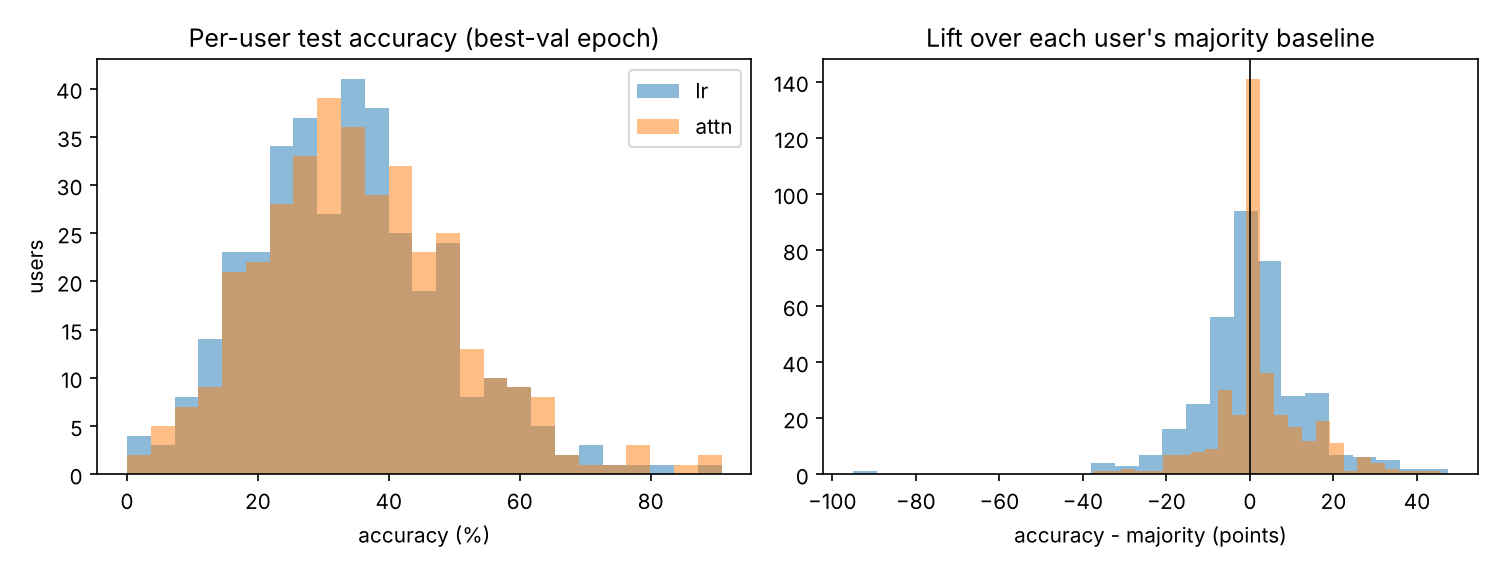
\includegraphics[width=\textwidth]{spread.png}
\caption{Per-user test accuracy (left) and lift over the majority baseline (right).}
\end{figure}

\section{Training time: plateau and optimum}
\begin{table}[h]\centering
\small
\begin{tabular}{lcccrr}
\toprule
 & \shortstack{Best epoch\\(median / mean)} & \shortstack{Optimal\\epoch} & Plateau & \shortstack{Test acc\\best-val} & \shortstack{Test acc\\epoch 300} \\
\midrule
LR & 71 / 95 & 85 & from epoch 58 & 33.7 & 33.6 \\
Transformer & 6 / 11 & 15 & none, then declines & 35.4 & 31.1 \\
\bottomrule
\end{tabular}
\caption{Optimal epoch is the maximum of the cross-user mean validation accuracy; plateau is the first epoch from which that mean stays within 0.5 points of its maximum for 10 epochs.}
\end{table}
More training does \emph{not} help the transformer: its mean validation accuracy is highest in the first few
epochs and then declines, and 300-epoch test accuracy is 4.3 points below the best-validation checkpoint
(paired difference vs.\ LR flips from $+1.7$ to $-2.5$). LR is the opposite: it climbs from 23\% to a plateau by about epoch 58 and
stays flat. The best training time is therefore short for the transformer (about 15 epochs, chosen per user by
validation loss) and about 60 to 85 epochs for LR. The extra capacity of the transformer overfits each user's
small training set.

\begin{figure}[h]\centering
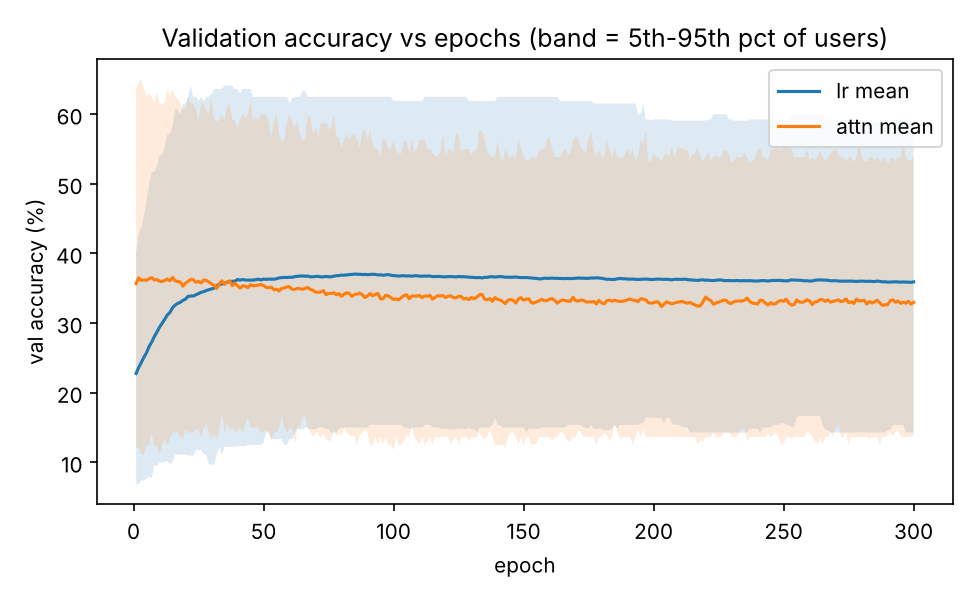
\includegraphics[width=0.75\textwidth]{val_acc_vs_epochs.png}
\caption{Mean validation accuracy versus epoch; the band is the 5th to 95th percentile across users.}
\end{figure}

\section{Effect of removing users with 100 or fewer ratings}
\begin{table}[h]\centering
\small
\begin{tabular}{lrrcr}
\toprule
 & Users & \shortstack{Median\\test size} & \shortstack{Accuracy std\\(LR / Transf.)} & \shortstack{Transf.\\lift} \\
\midrule
More than 100 ratings & 361 & 27 & 14.8 / 15.2 & $+2.5$ \\
100 or fewer ratings & 516 & 6.5 & 24.1 / 25.4 & $+0.2$ \\
\bottomrule
\end{tabular}
\caption{Kept versus dropped users (582 users have 100 or fewer ratings; 533 of them have at least 10 distinct timestamps, and 17 of those still could not be split chronologically, leaving 516).}
\end{table}
The filter mainly removes noise: dropped users have a median of 6.5 test ratings (as few as 1), so their accuracy
swings widely (standard deviation about 25 versus 15 points). The difference in lift between the two groups is
$+2.4$ points for the transformer ($[-0.4, +5.1]$) and $+2.2$ for LR ($[-1.1, +5.3]$); neither is significant at
99\%, so we cannot claim the filter raises accuracy, only that it gives cleaner and less variable estimates.

\section{Movie synopsis context}
The synopsis experiment is implemented (one extra context token built from a TF--IDF/SVD synopsis vector, $D=16$,
compared with genre-only models on identical users, splits and seeds) and tested for correctness, but
ml-100k contains no plot text. \textbf{Results are pending a synopsis file} (title, year, plot).

\section{Why did the paper not use deep neural networks?}
Based on the paper's own framing, there are three reasons, none of them that deep models predict better.
\emph{First}, the goal is not only prediction but \emph{optimizing} over the model's output in real time (choosing
the best set of items among catalogs of up to hundreds of millions, in milliseconds). For general transformers this
optimization is NP-hard, so the authors restrict to a simple single-layer transformer for which they prove a
near-optimal, sub-linear-time algorithm. \emph{Second}, this restriction is argued to cost little accuracy: the
paper reports the one-layer model about 2.5\% below the average general (multi-layer) transformer, and on the Spotify data
0.702 accuracy versus 0.704 for two layers and 0.726 for three (Sec.~5.1; figures as summarized from the paper's HTML
version, worth a check against its Table~1). \emph{Third}, the analysis assumes a small embedding dimension, which holds in practice. Our own results are
consistent with the accuracy point: on small per-user data, extra capacity overfits, so a larger network would
not help here either.

\section{Limitations and next steps}
Per-user test sets are small (median 27 ratings), accuracy is dominated by each user's majority class, and genre
flags carry little signal. Next: run the synopsis experiment once plot data is available, add richer features, and report accuracy as lift over the majority baseline throughout.

\end{document}
